\documentclass[10pt]{beamer}

\usetheme{Montpellier}
\usecolortheme{whale}

\usepackage[T1]{fontenc}
\usepackage{lmodern}

\usepackage{mathtools}
\usepackage[binary-units]{siunitx}
\usepackage{amsmath}
\usepackage{listings}
\usepackage{mdframed}
\usepackage{adjustbox}
\usepackage{minted}
\usepackage{xcolor}

\usepackage{parskip}
\usepackage{substr}
\usepackage{hyperref}
\usepackage{etoolbox}
\usepackage{tipa}
\usepackage{cprotect}
\usepackage{booktabs}
\usepackage{silence}
\usepackage[backend=biber, style=ieee]{biblatex}
\usepackage[english,ngerman]{babel}
\usepackage{csquotes}

\definecolor{lg}{gray}{0.95}
\hypersetup{colorlinks = true, urlcolor=blue, linkcolor=white}
\WarningFilter{biblatex}{Patching footnotes failed}

\renewcommand*{\bibfont}{\tiny}
\renewcommand{\subsectionname}{AA}

\bibliography{resources.bib}

\title{\textbf{Operating Systems}}
\subtitle{Tutorial 9}
\author{Fabian Klopfer}
\date{\today}

\defbeamertemplate{subsection page}{mine}[1][]{%
  \begin{centering}
    {\usebeamerfont{subsection name}\usebeamercolor[fg]{subsection name}#1}
    \vskip1em\par
    \begin{beamercolorbox}[sep=12pt,center]{part title}
      \usebeamerfont{subsection title}\insertsubsection\par
    \end{beamercolorbox}
  \end{centering}
}

\defbeamertemplate{section page}{mine}[1][]{%
  \begin{centering}
    {\usebeamerfont{section name}\usebeamercolor[fg]{section name}#1}
    \vskip1em\par
    \begin{beamercolorbox}[sep=12pt,center]{part title}
      \usebeamerfont{section title}\insertsection\par
    \end{beamercolorbox}
  \end{centering}
}

\setbeamertemplate{section page}[mine]
\setbeamertemplate{subsection page}[mine]

\begin{document}
\frame{\titlepage}


\begin{frame}{Intro}
\begin{itemize}
 \item Pingo Polls
 \item inofficial list of exam-relevant exercises
 \item Preview sheet 8
 \item Linking
\end{itemize}
\end{frame}

\begin{frame}{\alert{Inofficial} exam-relevant exercises list}
 Union of tasks \& questions considered relevant by Max \& Fabian. \vspace{0.3cm} \\
 Official list/sample exam to follow soon. \vspace{0.5cm} \\
 Comprehension questions: 
  \begin{itemize}
  \item 1.1.1, 1.1.3-4, 2.1.2-4, 2.1.6, 2.4.3-5, 2.4.7, 3.1.1, 3.1.3, 4.1.1-4, 4.1.7, 5.1.1-2, 5.1.4-9, 6.1.2, 6.1.4-8, 7.1.2, 7.1.5, 7.1.7
 \end{itemize}
 
 Exercises:
 \begin{itemize}
  \item 1.4, 2.2, 2.3, 3.3, 3.4, 4.3, 4.4, 4.5, 5.2, 5.3, 5.4, 5.5, 6.2, 6.3, 6.4, 6.5, 7.2, 7.3, 8.2, 8.3, 8.4
 \end{itemize}

\end{frame}


\section*{Exercise sheet 8}
\frame{\sectionpage}
\begin{frame}[allowframebreaks, fragile]{}
 \begin{figure}
           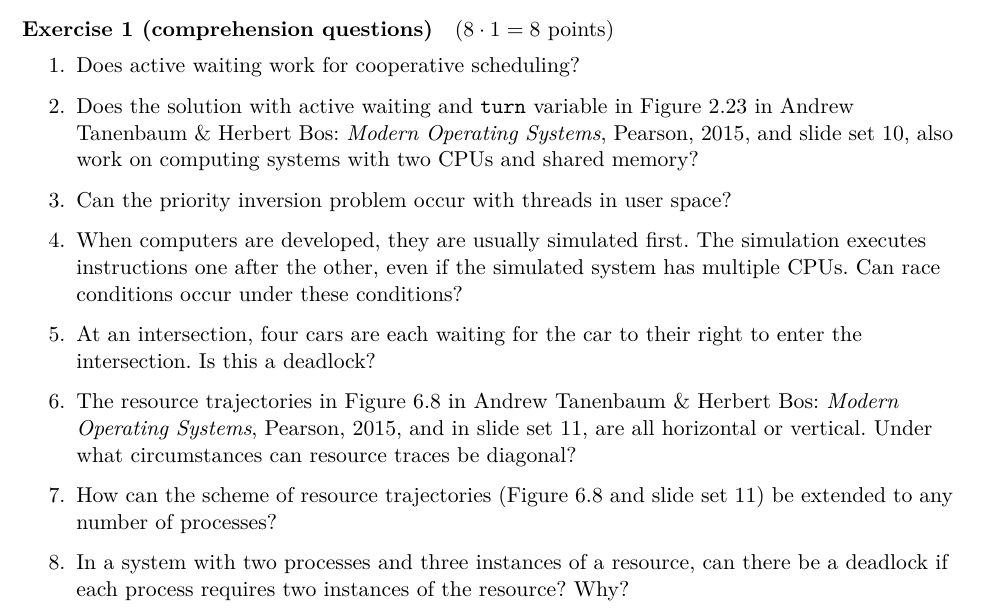
\includegraphics[keepaspectratio, width=\textwidth, height=\textheight-2\baselineskip-2\baselineskip]{img/ex8_100.png} \\
        \end{figure}
        \framebreak
        \begin{itemize}
         \item Cooperative scheduling $\Rightarrow$ process needs to yield! Does active waiting yield?
         \item Shared memory means both processes can access the variable
         \item What scheduling type do user level threads use (usually)?
         \item Can race conditions appear on a single threaded processor? Think about scheduling.
         \item Who is waiting for whom/what? Draw the diagram.
         \item Shaded areas mark intersections. What do diagonals stand for in terms of execution?
         \item Here two processes are the x and y axis respectively
         \item Can a circular wait occur?
        \end{itemize}
        \framebreak
        
  \begin{figure}
          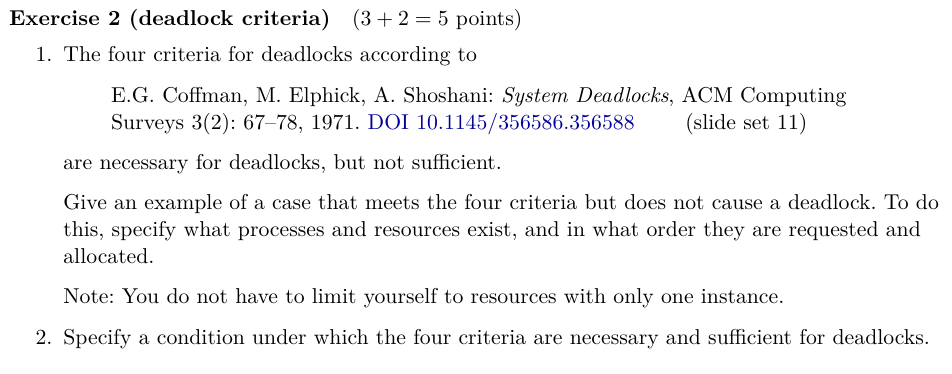
\includegraphics[keepaspectratio, width=\textwidth, height=\textheight-2\baselineskip-2\baselineskip]{img/ex8_101.png} \\
        \end{figure}
        \begin{itemize}
         \item It has to do with if a resource is unqiue or can have multiple instances (e.g. a printer spooler)
         \item as above
         \end{itemize}
        \framebreak
        
         \begin{figure}
          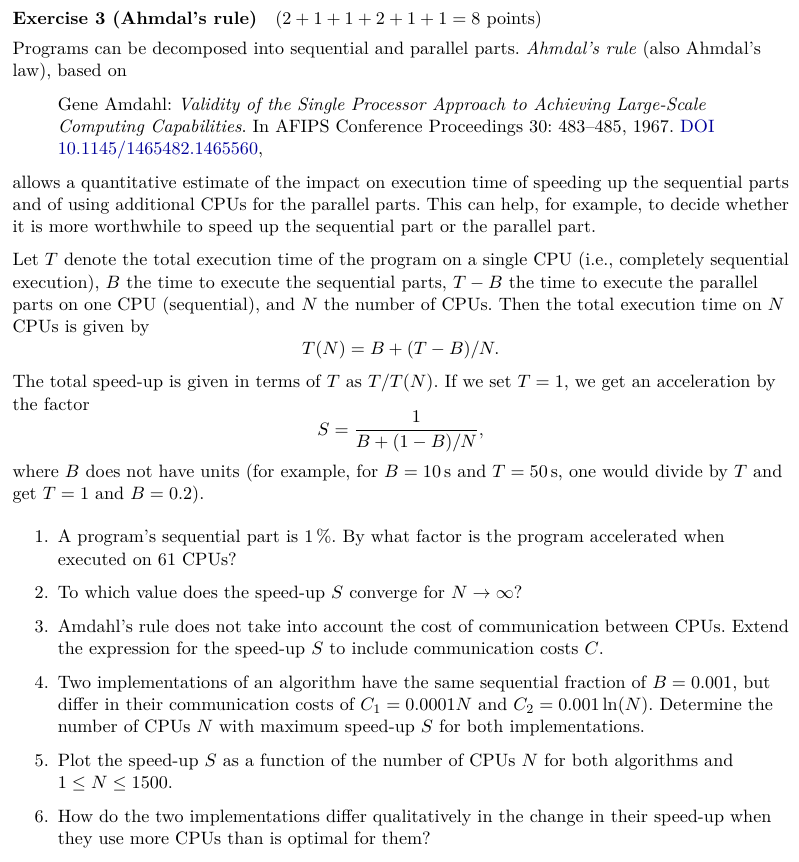
\includegraphics[keepaspectratio, width=\textwidth, height=\textheight-2\baselineskip-2\baselineskip]{img/ex8_102.png} \\
        \end{figure}
        \framebreak
        \begin{itemize}
         \item Read carefully
         \item take the limit
         \item To what do the communication costs contribute to?
         \item Similar to 6.5.3 in terms of the steps
         \item depends on the communication costs
        \end{itemize}
        \framebreak 
        
         \begin{figure}
          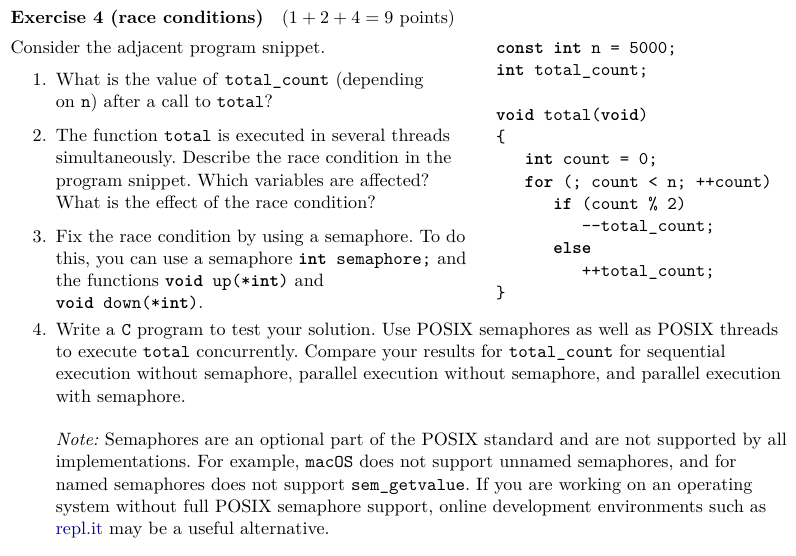
\includegraphics[keepaspectratio, width=\textwidth, height=\textheight]{img/ex8_103.png} \\
        \end{figure}
        \begin{itemize}
         \item Do this properly! Esp. 2) is a popular exam question.
        \end{itemize}
        \framebreak 
\end{frame}

\section*{Linking}
\frame{\sectionpage}
    

\section{References}
    \begin{frame}[allowframebreaks]
      \frametitle{References}
      \begin{tiny}
      \nocite{*}
      \printbibliography
      \end{tiny}
    \end{frame}


\end{document}
 
